%% This represents the Master-File of ZwickTeX-Template
%% END of Header
%~~~~~~~~~~~~~~~~~~~~~~~~~~~~~~~~~~~~~~~~~~~~~~~~~~~~~~~~~~~~~~~~~~~~~~~~~~~~~~~~~


%%%
% Mögliche Klassen-Optionen:
%  noindex -> Keinen Index erstellen
%  noabbrevlist -> Kein Abkürzungsverzeichnis
%  nolistoflists -> Kein Listings-Verzeichnis
%  nolistoftables -> Kein Tabellenverzeichnis
%  nolistoffigures -> Kein Abbildungsverzeichnis
%  noappendixtoc -> Kein Anhangsverzeichnis
%  nomarginnotes -> Alle Randnotizen ausblenden
% ... plus die KOMA Klassenoptionen für scrreprt
\documentclass[]{zwicktex}
%% This is file Abkuerzungen.tex of ZwickTeX-Template
%% END of Header
%~~~~~~~~~~~~~~~~~~~~~~~~~~~~~~~~~~~~~~~~~~~~~~~~~~~~~~~~~~~~~~~~~~~~~~~~~~~~~~~~~


%% Abkürzungen zur Verwendung im Text
%% Aufruf im Text: \gls{<Textmarke>}
%% Wir beim ersten mal automatisch ausgeschrieben, die weiteren Male abgekürzt
%% Schema: \newacronym{<Textmarke>}{<Abkürzung>}{<Ausgeschrieben>}

\newacronym{abk}{Abk.}{Abkürzung} %HINWEIS: Speziell DIESER Eintrag sollte gelöscht werden^^
\newacronym{aeg}{AEG}{Ausschalten Einschalten Geht}
\newacronym{ddr}{DDR}{Deutsche Dominikanische Republik}



%~~~~~~~~~~~~~~~~~~~~~~~~~~~~~~~~~~~~~~~~~~~~~~~~~~~~~~~~~~~~~~~~~~~~~~~~~~~~~~~~~
%% EOF Abkuerzungen.tex


%% This is file Trennvorschriften.tex of ZwickTeX-Template
%% END of Header
%~~~~~~~~~~~~~~~~~~~~~~~~~~~~~~~~~~~~~~~~~~~~~~~~~~~~~~~~~~~~~~~~~~~~~~~~~~~~~~~~~


%% Trennvorschriften zur Verwendung im Text

% \- : Immer an einer dieser Stellen trennen, Automatismen ignorieren: Staats\-ver\-trag.
% "- : Zusätzliche Trennstelle angegeben. Falls LaTeX das mal nicht richtig erkennt
% "= : Bindestrich, der Trennungen an anderen Stellen weiterhin erlaubt
% "" : Umbruch erlauben, ohne dass ein Bindestrich gesetzt wird (z.B. in Verbindung mit "=
% "~ : Bindestrich, an dem nicht getrennt oder umgebrochen werden soll


\hyphenation{Plau-si-bi-li-sierung Schwei-ne-pries-ter}


%% Bewirkt, dass die angegebenen Wörter im gesamten Text nur an den - Stellen getrennt werden




%~~~~~~~~~~~~~~~~~~~~~~~~~~~~~~~~~~~~~~~~~~~~~~~~~~~~~~~~~~~~~~~~~~~~~~~~~~~~~~~~~
%% EOF Trennvorschriften.tex




%%%
% Wichtigste Einstellungen
\setTitel{} 		% Titel der Arbeit
\setAutor[m]{} 		% Hier kommt Dein Name rein, und in eckigen Klammern Dein Geschlecht (m/w) für Titelseite
\setMatrNr{}		% Deine Matrikelnummer
\setThesis{} 		% Was für ne Arbeit? (Default ist Diplomarbeit)
\setAkadGrad{} 		% Zu erreichender Grad
\setBetreuer[m]{} 	% Name des Betreuers, und in eckigen Klammern das Geschlecht (m/w) für Titelseite
\setStudiengang{} 	% Dein Studiengang
\setDatum{\today} 	% Abgabedatum (Default ist heutiges Datum: \today)
\setKeywords{} 		% Deine Keywords, die evtl. im Summary später auftauchen (Zuletzt aufrufen!)

%%%
% Seitenränder ändern
%\geometry{left=3.5cm,right=3cm,top=3cm,bottom=3cm}%



%%%
% Jetzt geht´s los
%%+++++++++++++++++++++++++++++++++++++++++++++++++++++++++++++++++++++++++++++++++++++++++++++++++++++
 \begin{document}
%%-----------------------------------------------------------------------------------------------------
% AB HIER KEINEN INHALT EINFÜGEN !!! Dafür gibt es die Hauptteil.tex 1elf!

%%%
% Befehl um die Titelseite zu generieren
\Titelseite 


%%%
% Deine Erklärung an Eides statt
%% This is file Erklaerung.tex of ZwickTeX-Template
\begingroup
\addchap*{Eidesstattliche Erklärung}
\onehalfspacing
\normalsize
%% END of Header
%~~~~~~~~~~~~~~~~~~~~~~~~~~~~~~~~~~~~~~~~~~~~~~~~~~~~~~~~~~~~~~~~~~~~~~~~~~~~~~~~~





% Eidesstattliche Erklärung:

Ich erkläre hiermit, dass ich die vorliegende \getThesis\xspace selbständig und ohne
fremde Hilfsmittel verfasst und in der Bearbeitung und Abfassung keine anderen als
die angegebenen Quellen oder Hilfsmittel benutzt sowie wörtliche und sinngemäße
Zitate als solche gekennzeichnet habe. Die vorliegende Diplomarbeit wurde noch
nicht anderweitig für Prüfungszwecke vorgelegt.

\vspace{1em}

Kufstein, \today

\vspace{3em}

\getAutor







%~~~~~~~~~~~~~~~~~~~~~~~~~~~~~~~~~~~~~~~~~~~~~~~~~~~~~~~~~~~~~~~~~~~~~~~~~~~~~~~~~
%% BEGIN Footer
\endgroup
%% End of Footer
%% EOF Erklaerung.tex

 


%%%
% Einstellungen und Verzeichnisse im Vorspann aufführen
\Vorspann 
  %% This is file Kurzfassung.tex of ZwickTeX-Template
\begingroup
\onehalfspacing
%% END of Header
%~~~~~~~~~~~~~~~~~~~~~~~~~~~~~~~~~~~~~~~~~~~~~~~~~~~~~~~~~~~~~~~~~~~~~~~~~~~~~~~~~



% Kurzfassung Deutsch
\addchap{Kurzfassung}

%==============================================
FH Kufstein \\
\getStudiengang \\
Kurzfassung der \getThesis\xspace \getTitel  \\
\getAutor \\
\getBetreuer \\
Vorname Zweitbetreuername \\
%==============================================


Die Kurzfassung dient dem Aufbau einer internen Datenbank und der Weitergabe
von Informationen an Interessenten außerhalb der FH Kufstein.
Die Kurzfassung ist sowohl auf Deutsch als auch auf Englisch zu erstellen (2 Versionen).

Bei der englischsprachigen Kurzfassung muss auch der Titel der Diplomarbeit
in englischer Sprache angegeben werden. Die Kurzfassung sollte jeweils nicht mehr
als 1 Seite umfassen und im Fließtext mit möglichst wenigen Aufzählungen und ohne
Abbildungen, Fußnoten oder Formatierungen gestaltet sein. Sie soll in knapper Form \ldots

die Problemstellung, \\
die Zielsetzung, \\
die Methodik \\
und die wichtigsten Ergebnisse darstellen. 

Die Kurzfassung ist nach dem Abkürzungsverzeichnis und vor dem
eigentlichen Text in die Arbeit einzubinden sowie auf Datenträgern oder via E-Mail
mit den gebundenen Exemplaren der Diplomarbeit abzugeben. Die Kurzfassung soll
folgende Angaben enthalten:

1. Zeile, linker oberer Rand: FH Kufstein \\
2. Zeile: „[Studiengang]“ \\
3. Zeile: Kurzfassung der Diplomarbeit ... (Titel einfügen) \\
4. Zeile: Name des Studierenden \\
5. Zeile: Erstbetreuer \\ 
6. Zeile: Zweitbetreuer \\

Text der Kurzfassung – Fließtext, ca. 350 Wörter









%~~~~~~~~~~~~~~~~~~~~~~~~~~~~~~~~~~~~~~~~~~~~~~~~~~~~~~~~~~~~~~~~~~~~~~~~~~~~~~~~~
% Zusammenfassung Englisch
\addchap{Abstract}

%==============================================
FH Kufstein \\
\getStudiengang \\
Abstract of \getThesis\xspace Englischer Titel  \\
\getAutor \\
\getBetreuer \\
Vorname Zweitbetreuername \\
%==============================================


Same procedure as before\ldots









%~~~~~~~~~~~~~~~~~~~~~~~~~~~~~~~~~~~~~~~~~~~~~~~~~~~~~~~~~~~~~~~~~~~~~~~~~~~~~~~~~
%% BEGIN Footer
\endgroup
%% End of Footer
%% EOF Kurzfassung.tex

 % Deine Kurzfassungen auf Deutsch und Englisch


%%%
% Einstellungen für den Hauptteil
\Hauptteil 
  %% This is file Hauptteil.tex of ZwickTeX-Template
\begingroup
\onehalfspacing
%% END of Header
%~~~~~~~~~~~~~~~~~~~~~~~~~~~~~~~~~~~~~~~~~~~~~~~~~~~~~~~~~~~~~~~~~~~~~~~~~~~~~~~~~



%% Der Hauptteil: Hier schreibt Eure Arbeit rein. Dies sind die Seiten, die für die Arbeit zählen!

\chapter{Erstes Kapitel des Hauptteils}
 \section{Unterüberschrift}
  \subsection{Unterunterüberschrift}
   \subsubsection{Unterunterunterüberschrift}

%% ENTFERNE DIES:
%% This is file examples.for.template.tex of ZwickTeX-Template
%% END of Header
%~~~~~~~~~~~~~~~~~~~~~~~~~~~~~~~~~~~~~~~~~~~~~~~~~~~~~~~~~~~~~~~~~~~~~~~~~~~~~~~~~


% NUR FÜR TESTZWECKE!!! 
% Hiermit provoziert man die Erstellung eines vollständigen Literaturverzeichnises ALLER BibTeX DB-Einträge
% Sollte entfernt werden!
\nocite{*} 	
%%%



\chapter{Geleitwort und Verwendung}
\label{kap:Geleitwort}

Diese Vorlage soll Dir einen Schnellstart für die Verwendung von \latex für Deine Abschlussarbeit ermöglichen.  Sie kommt in einer bestimmten Zusammenstellung, mit der Du eigentlich sofort loslegen kannst. Wenn Du Dinge verändern willst, so läuft das auf eigenes Risiko, aber ich habe darauf geachtet, den Code relativ leicht verständlich zu halten. Dadurch sollte individuelles Customizing leicht möglich sein. Beachte aber, dass die Konfiguration, so wie sie vorliegt, mit der Studiengangsleitung abgestimmt wurde.

\section*{ZwickTeX und Hauptdokument}

Kern des Ganzen ist das Hauptdokument \texttt{Zwickmaster-fat-2012.tex} im Wurzelverzeichnis. Dieses kannst Du nun - im Gegensatz zu meiner alten BA-Vorlage von 2009 - ganz nach Belieben umbenennen, ohne dass die Funktionsweise beeinträchtigt wird. Allerdings habe ich mich bemüht, dass die Rückwärtskompatibilität (weitestgehend) gegeben ist.

Darin wird die Klasse \zwicktex\xspace aufgerufen, die in Würdigung eines Profs so benannt wurde, der sich uns gegenüber vor langer Zeit als \LaTeX-Fetischist geoutet hatte… ~;-)

\subparagraph*{Hinweis:} Ein Branch der alten BA-Vorlage ist hier zu finden: \\
\url{https://github.com/maff/latexpaper-clean/tree/master/src}

Diese Klasse ist kein Hexenwerk, sondern ist von mir relativ hemdsärmelig gecodet worden. Sie ist vollgepackt mit einem Haufen Paketen, so dass Ihr für die meisten Dinge gerüstet sein solltet. 

Ein besonderes Gimmik meiner Klasse ist, dass die sonst nötigen abwechselnden Aufrufe von \texttt{pdflatex}, \texttt{bibtex} und \texttt{makeindex} hier nicht nötig sind! Das erledigt die Klasse automatisch. (s.a. Kap. \ref{lab:shellescape})

\subparagraph*{Wichtig!} Das PDF wird erst nach viermaligem(!) Aufruf von PDFLaTeX (per TeXmaker) vollständig erstellt! 

\subparagraph*{Hinweis:}  \midx{\zwicktex} baut auf der \midx{KOMA}-Klasse \texttt{scrreprt} auf, und leitet Klassenoptionen dahin weiter. Seitenränder werden über das \texttt{geometry}-Paket gesetzt. Google hilft.

\subparagraph*{Hinweis:}  Schau dir die Doku der \midx{KOMA}-Klasse an, den \verb|scrgiude|. Dort wird so einiges erklärt: \\
\url{http://mirror.ctan.org/macros/latex/contrib/koma-script/doc/}

Mit den folgenden Hinweisen und einer Portion gesundem Menschenverstand hast Du alles, was an Werkzeugen nötig ist. Auf den folgenden Seiten findest Du dann noch Beispiele (s. Kap. \ref{kap:beispiele}) und Hinweise zur Benutzung dieser Vorlage, aber erwarte keinen \latex Kurs.
Der Rest liegt an Dir! Viel Erfolg wünsche ich, und wenn Dir das Template gefällt, gib bitte Dein Wissen und die gewonnene Erfahrung an die Folge-Jahrgänge weiter.


\section*{Ordner und Dateien}
Ein gut gemeinter Rat: Behalte die vorgesehene Datei- und \midx{Ordnerstruktur} bei, und Du ersparst dir einiges an Frustration.

\verb|\config| enthält notwendige Konfigurationsdateien. \\
\textbf{(Hier dürfen die Dateinamen nicht geändert werden!)}

\verb|\inhalte| soll deine Inhalte (Texte) aufnehmen.

\verb|\graphics| ist der Standardpfad für Grafiken.

\verb|CLEAN-TMP.bat| ist eine Batch-Datei auf oberster Ebene. Die säubert das Verzeichnis von temporären Dateien, was manchmal bei undurchsichtigen Fehlern hilfreich sein kann, oder bevor Ihr eine Sicherung erstellt.


\section*{Handhabung (Quick Start)}
Der Zwickmaster ist Dein Hauptdokument. Trage dort als erstes Deine persönlichen Daten ein, \textbf{und vergiss nicht die Geschlechtsangaben bei Dir selbst und deinem Betreuer!}

Als nächstes entferne die Beispiel-Inhalte, indem Du im Master das Einbinden der Examples-Datei entfernst oder auskommentierst.

Dann erst kümmere Dich um die restlichen Inhalte, die Du in die vorgesehenen Dateien und Ordner einfügst.


\chapter{Stuff you need}
\label{kap:stuffuneed}

Für die Verwendung dieser Vorlage empfehle ich hier ein paar Tools, mit denen Du gut zurechtkommen solltest, und ziemlich schnell zu brauchbaren Ergebnissen kommst. Das \zwicktex-Template ist dafür ausgelegt, und funktioniert mit den aktuell gebräuchlichen Versionen einwandfrei.

Bitte sieh zu, dass Du die genannte Software in der aufgeführten Reihenfolge installierst. Es steht Dir frei, mit anderen Tools zu experimentieren, und dir so viele komische Fehler ins Haus zu holen, wie Du willst...

Sobald Du alles auf Platte hast, schmeiß den Kompiliervorgang für das Hauptdokument an, so wie es aus dem Archiv kommt. Es sollte dabei alles ohne Fehler vonstatten gehen.

\subparagraph*{Wichtig!} Rechne damit, dass beim ersten Anwerfen des Kompilierungs-Vorgangs abhängig von Leistung und Internetz-Anbindung bis zu 30 Minuten vergehen können, bis alles geladen wurde! \\
(Danach ists eine Sekundensache.)




\section*{MikTeX}
Zuerst die \LaTeX-Umgebung, unter Windows gibt’s da eigentlich nur eine: \midx{MikTeX}

\url{http://miktex.org/}

\subparagraph*{Hinweis:} Installiert MikTeX bitte so, dass fehlende Pakete automatisch nachinstalliert werden.  Dazu den richtigen Installer auswählen! Ich nutze "Basic MiKTeX 2.9" Installer.




\section*{TeXmaker}
Da wir hier ausschließlich mit \midx{UTF-8} Zeichencodierung arbeiten, und das (stabile) \midx{TeXnicCenter} so einen neumodischen Kram (sic!) immer noch nicht unterstützt, hol Dir den \midx{TeXmaker}, einen sehr guten und schlanken Editor für \latex mit Out-of-the-box Rechtschreibkorrektur.

\url{http://www.xm1math.net/texmaker/}

\subparagraph*{Hinweis 1:} Konfiguriere ihn bitte gleich so, dass die Standard-\midx{Zeichencodierung} auf UTF-8 eingestellt ist. Bei unterschiedlichen Zeichenkodierungen können deine Dateien zerstört werden!
\subparagraph*{Hinweis 2:} Die wichtigste Taste findest Du oben in der Mitte (s. Abb. \ref{fig:texmakerstart} auf Seite \pageref{fig:texmakerstart}). Das startet nach Auswahl von \texttt{PDFLaTeX} den Kompilierungs-Vorgang.
\subparagraph*{Hinweis 3:} Bitte passt den Aufruf von MikTeX in TeXmaker an, um die automatischen Aufrufe von u.a. \verb|makeindex| zu ermöglichen. Geht dazu in die Einstellungen, und setzt den \label{lab:shellescape}
Sring bei PdfLaTeX auf \\
 \verb|pdflatex -interaction=nonstopmode --shell-escape %.tex|

\bigskip
\begin{figure}[h!] % Mit 'H' wird noch extremer versucht, das Objekt direkt HIER zu setzen, alternativ 'h!'
	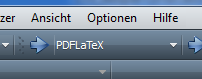
\includegraphics[width=0.3\textwidth]{TeXmaker1} 		% Bild relativ zur Textbreite skalieren
	\caption[Dieser Text erscheint nur im Verzeichnis]%
			{Zuerst im Dropdown PDFLaTeX auswählen, und dann mit Klick auf den blauen Pfeil den Kompilierungs-Vorgang starten. (Quelle: Screenshot von TeXmaker 2.3 unter Windows 7)}
  	\label{fig:texmakerstart}
\end{figure}
\bigskip




\section*{Grafiken}
\label{sec:Grafiken}
Wenn Du in Word Bilder einfügen möchtest, so kommst Du in der Regel um Pixelgrafik wie z.B. \midx{JPEG} oder \midx{PNG} nicht herum (Komm mir nun bitte nicht mit BMP oder TIF!). 

Diese Formate können in \latex freilich auch eingebunden werden, aber wer auf gute Qualität steht, der verwendet \midx{Vektorgrafik}. Die bietet bei egal welcher Auflösung immer optimale Qualität, und kommt gestochen scharf aufs Papier oder den Bildschirm. Außerdem kannst Du die ohne Verluste auf das benötigte Format skalieren. 

\subparagraph*{Hinweis:} Das FH-Logo für die Titelseite habe ich Euch schon als Vektorgrafik besorgt. Da kann Word leider nicht mithalten…  ~:-P \\
Bitte sei Dir bewusst, dass dieses Logo mit Copyright belegt ist. Verteile es also nicht außerhalb der FH weiter!



\subsection*{PDF-Grafiken erstellen}
\label{PDF-Grafik}
Das bedeutet also für Dich, dass Du wo es irgend geht mit PDFs arbeiten wirst. Das ist heutzutage extrem einfach. Als kleinen „Cheat“ empfehle ich, \midx{Tabellen} in \midx{Excel} zu erstellen, und dann direkt aus MS Office heraus als PDF abzuspeichern. 

Wo das direkte Abspeichern nicht funktioniert, da benutze einen PDF-Drucker. Damit druckst Du wie gewohnt aus (fast) jeder Anwendung eine \midx{Vektorgrafik}, und auch aus MiniTab kommen hübsche Diagramme in deine Arbeit. \\
Ein guter und schlanker \midx{PDF-Drucker} ist FreePDF:

\url{http://freepdfxp.de/}



\subsection*{PDF zuschneiden mit BRISS}
Da kommen wir dann zum nächsten Punkt: So ein gedrucktes PDF hat für gewöhnlich weiße \midx{Ränder}, die wir nicht gebrauchen können. 

Wer sich den Adobe Acrobat nicht leisten möchte, findet eine elegante, schlanke und freie Variante die Ränder loszuwerden, in Briss: Ein Java-basiertes Tool ohne Installations-Orgien, mit grafischer Oberfläche.

\url{http://sourceforge.net/projects/briss/}

\section*{Literaturverwaltung} \index{Literaturverwaltung}
Damit seid Ihr schon ziemlich gut gerüstet, und könnt fast schon loslegen. Da bleibt nur noch ein großes Thema: Die Literatur.

Ich empfehle mittlerweile, die Software \verb|citavi| zu verwenden! Davon gib es eine Freeware Version, die immerhin 100 Titel verwalten kann. Wem das nicht reicht, der hat vielleicht Glück, und bekommt es kostenlos über eine Campuslizenz (derzeit leider noch nicht in Kufstein, aber z.B. die Uni Innsbruck ist vertreten.) \\
Mehr als 4000 (sic!) Online Kataloge sind abrufbar, sie findet selbständig einige lizenzpflichtige Datenbanken, solange Du dich im Netz der Hochschule befindest. Dokumentenmanagement und Aufgabenplanung sind ebenso drin, wie ein Plugin für Firefox und Internet Explorer.

Geil: Über einen Shortcut kannst Du direkt den Cite-Key für \latex bzw. \bibtex in deinen TeXmaker übernehmen, und das sogar selbst definieren. Beispielsweise kannst Du ihm direkt sagen, dass Du in einer Fußnote zitieren willst, und mit einem Klick hast Du den entsprechenden \latex Code in Deinem Dokument (z.B. habe ich dies hier mit $Strg+W$ eingefügt: \verb|\footnote{\citep[vgl.][]{Griesbaum.2010}|)

Ausgewählte Titel -- oder die ganze Sammlung -- kannst Du dann als \bibtex Bibliothek exportieren, in den Ordner Deiner Arbeit speichern, und los gehts\dots

Zuvor habe ich auf das kostenlose \midx{JabRef} gesetzt, aber es hat mich zu oft enttäuscht. Wollt Ihr etwas noch ganz anderes verwenden, so achtet nur darauf, dass das \bibtex-Format unterstützt wird.

\url{http://www.citavi.com/de/}

\subparagraph*{Hinweis:} Für JabRef gibt es z.B. die  Möglichkeiten, aus Amazon-Einträgen  \midx{\bibtex} Code ausgeben zu lassen, und auch Google-Scholar bietet das an. \\
\verb|Citavi| macht das hundertmal besser, und direkt aus dem Programm heraus aus tausenden Quellen.








\chapter{Beispiele}
\label{kap:beispiele}


\section{Abkürzungen}
Die Abkürzungen werden in der entsprechenden Datei im Ordner "Contents" definiert.

Bei der Verwendung im Text wird nur die Textmarke angegeben. Dadurch wird bei der ersten Verwendung im Text die Langform mit der Abkürzung in Klammern ausgegeben, als dann stets die Kurzform.

Erste Verwendung: \gls{ddr}

Nachfolgende Verwendung: \gls{ddr}

Beide Aufrufe erfolgten mit \verb|\gls{ddr}|




\section{Zitate und Quellenverweise}
%%
\subsection{Generelles zum Zitieren in dieser Vorlage}
\url{http://de.wikibooks.org/wiki/LaTeX-Kompendium:_Zitieren_mit_BibTeX}

%%
\subsection{Wörtliches Zitat mit Herausstellung}
	\verb|\begin{zitat}[S.123]{BibTeXkey}| \\
    \verb|<Zitattext>| \\
	\verb|\end{zitat}|\\
\begin{zitat}[S.123]{testbook} % VORSICHT: Zuerst eckige Klammern für optionale Seitenangabe, dann geschweifte Klammern
	Wörtliche Zitate werden durch einen linken und rechten Einzug von jeweils 1 cm
	und kursiven Schriftstil kenntlich gemacht. Das Zitat wird in Anführungszeichen gesetzt.
	Anschließend muss die Quelle angegeben werden.	
\end{zitat}

%%
\subsection{Normales (indirektes) Zitat mit Fußnote}
	\verb|\footcite[S.365ff]{testbook}|
	
	So zielt Gesundheitserziehung darauf ab, vorgegebene Einstellungen, Fähigkeiten
	und Fertigkeiten sowie Kompetenzen zu vermitteln.\footcite[S.365ff]{testbook} \\

%%%%%
\subsection{Zitation im laufenden Text}
	\verb|\citet[S.365ff]{testbook}|
	
	Dies bestätigten \citet[S.365ff]{testbook} mit diversen ...
	
\subsection{Hilfestellung Quellenverweise für Bilder}

\verb|\citefigure{S.123}{key}|:~ \citefigure{S.123}{ritscheltirol2010}

\verb|\citefigureown|:~\citefigureown 

\verb|\citefiguremodified{S.32}{key}|:~\citefiguremodified{S.32}{schlosserwissenschaftliche2011}

\verb|\citefiguredata{124}{key}|:~\citefiguredata{S.124}{kaiserkufstein2010}











\section{Häufige Sonderzeichen und Symbole}
\label{sec:Sonderzeichen}

\latex bietet viele hübsche Symbole an, die teils nach geometrischen Verhältnissen erst beim Aufruf generiert werden (z.B. das Euro-Symbol). Durch diesen Umstand wurde es speziell für den Umgang mit mathematischen Formeln sehr berühmt (kleines Beispiel folgt sogleich). Geht aber davon aus, dass Ihr fast alles verwenden könnt, was ihr im Internetz findet: Diese Vorlage ist ziemlich dick ausgestattet, und bindet Euch schon einen Haufen Fonts dafür ein. Den Rest holt Euch über Packages in der Präambel.
	
\[ \frac{\sum_{i=1}^{n} \left( \frac{1}{r} \right)^{\ell_i} \leq 1}{\sum \limits_{i=1}^n i = \frac{n(n+1)}{2}} \]
	
Ich zeige Euch ein paar häufig verwendete \midx{Symbole}, und die zugehörigen Befehle in Tabelle \ref{tab:Sonderzeichen}. Um übrigens \LaTeX-Code nicht ausführen, sondern darstellen zu lassen, benutze ich eine \verb|\verb| Umgebung.
Was ich nicht explizit anführe, guckt Euch einfach im Sourcecode dieser Beispieldatei ab.
	
\midx{Sonderzeichen} auf der Tastatur werden meist als \midx{Steuerzeichen} interpretiert. Um sie zu verwenden, genügt aber oft schon ein vorangestellter Backslash: \verb|\$| \verb|\%| \verb|\&|


\begin{table}[h!]
\caption[Sonderzeichen]{Eine kleine Auswahl an Sonderzeichen}
\label{tab:Sonderzeichen} 	% Textmarke
\centering
\begin{tabular}{p{0.08\textwidth}p{0.22\textwidth}p{0.57\textwidth}}
\hline
 ,, ``          & \verb|,, ``| & Anführungszeichen: 2 x Komma für unten, 2 x Shift-Akzent für oben; TIPP: Copy´n´Paste aus Word \\
 \mtrade        & \verb|\mtrade| & Trademark\mtrade \\ 
 \mcopy         & \verb|\mcopy| & Copyright\mcopy \\ 
 \mregistered   & \verb|\mregistered| & Registered\mregistered \\ 
 \euro          & \verb|\euro| &  \\ 
                & \verb|\EUR{10}| & zeigt \EUR{10} mit korrektem schmalem Zeichenabstand \\ 
 \promill       & \verb|\promill| & Promille \\ 
 \cpluspluslogo & \verb|\cpluspluslogo| &  \\ 
 \celsius       & \verb|\celsius| &  \\ 
 \textdegree    & \verb|\textdegree| & Grad, auch Winkelgrad \\ 
 \O             & \verb|\O| & Durchschnitt: Backslash und großes O \\ 
 \sixsigma      & \verb|\sixsigma| & \midx{Six Sigma} \\ 
\hline
\end{tabular} 
\end{table}
	



\section{Referenzieren im Text}
\label{sec:Referenzen}
\index{Referenzen}
\index{Verweise}
\index{Bezüge}

Im laufenden Text kannst Du auf all jene Stellen im Text referenzieren, denen Du vorher ein
\verb|\label{Textmarkenname}| zugewiesen hast.

Das ist besonders hilfreich für Bilder, Tabellen oder Kapitel und Abschnitte.

Auf ein Bild referenzieren (d.h. die Abbildungs-Nummer ansprechen):\\
 \verb|\ref{fig:texmakerstart}| \\
(Das führende fig: ist mein persönlicher Geschmack zur Übersicht!)

Und die Seitenzahl des Bildes: \verb|\pageref{fig:texmakerstart}|

Das führt uns zu Abbildung \ref{fig:texmakerstart} \\
auf Seite \pageref{fig:texmakerstart} \\
(Zahlen werden Hyperlinks!)

Analog dazu läuft es mit \midx{Labels} von Tabellen oder Textstellen.


\begin{myfloatbox}[caption={myfloatbox-Testlisting},label={lst:Beispiellisting3}]
Auf mich  musst Du im Text verweisen,
denn Meinereiner geht auf Reisen.
Nun guck nicht lang was ich hier wollte,
lies weiter was mich hierher rollte.
\end{myfloatbox}



\subparagraph*{Hinweis:} Sollten Bezüge (oder Quellenverweise) beim Kompilieren nur als Fragezeichen dargestellt werden, liegt das oft daran, dass nicht alle Kompilierungs-Läufe gemacht wurden, oder die Daten nicht konsistent sind (falsche oder fehlende Labels?). Guckt dann genau in die Logs.)

\subparagraph*{Wichtig:} Bilder müssen von \verb|\begin{figure}[!h]| und \verb|\end{figure}| umschlossen sein, Tabellen (auch als PDF eingefügte Excel-Tabellen!) mit \verb|\begin{table}[!h]| und \verb|\end{table}| umschlossen sein. Nur so werden sie auch in den Listen und Verzeichnissen aufgeführt! (Siehe Beispiel-Datei; das \verb|!h| bedeutet, dass \latex dieses Ding möglichst HIER setzen soll.)

Wenn Ihr eine Excel-Tabelle als PDF einfügt, so achtet darauf, welcher Tag die Caption klammert. Diese Klammer (entweder \verb|figure| oder \verb|table|) entscheidet, ob es als Tabelle oder Bild erkannt wird.

Ein Beispiel findest Du in Listing \ref{lst:ExcelTabelle}.

\begin{mycodebox}[caption={Einbinden von Tabellen die als PDF vorliegen},label={lst:ExcelTabelle},language=TeX]
\begin{table}[!h]
 \caption[CaptionFürListing]{Caption die direkt über der Tabelle auftaucht}
 \label{tab:Textmarkenname} 	% Textmarke
 \centering
  %%Jetzt erst die eigentlich Tabelle als PDF
   \begin{figure}
	\includegraphics[width=0.3\textwidth]{Exceltabelle.pdf} 
   \end{figure}	
\end{table}
\end{mycodebox}




\section{Index-Einträge}
\label{sec:Indexzeug}
\index{Index}

Ganz am Ende dieses Dokumentes findest Du einen Index (abschaltbar über Klassenoption!). Das ist vielleicht etwas ungewöhnlich, für mich selbst jedoch habe ich festgestellt, dass ich dadurch bei der Erstellung leichter den Überblick bewahren kann.

Beim Schreiben setze ich an prägnanten Punkten einfach ein \verb|\midx{Wort}| in den Text. Das Wort erscheint ganz normal im Text, und zusätzlich wird es im Index aufgeführt und verlinkt. Soll nur ein "unsichtbarer" Anker für einen Indexeintrag erstellt werden, so geht das mit \verb|\index{Wort}|, wobei hier das Wort aber nicht an dieser Stelle im Text erscheint, sondern nur im Index mit Bezug auf genau diese Stelle.





\section{Einfache Listen und Aufzählungen}
\label{sec:Listen}
\index{Aufzählungen}

Einfache Listen und Aufzählungen erstellt man (auch geschachtelt) mit \verb|\begin{itemize}| oder \verb|\begin{enumerate}|:

\begin{onehalfspacing}
\begin{itemize}
\item Bla bla
\item Blubb
	\begin{itemize}
	\item Buh
	\item Bäh
	\begin{enumerate}
		\item Eins
		\item Zwei
		\item Drei
	\end{enumerate}
	\item Bam
	\end{itemize}
\item Pfui
\end{itemize}
\end{onehalfspacing}







\section{Codelistings}
\label{sec:codelist}

\begin{mycodebox}[caption={mycodebox-Testlisting},label={lst:Beispiellisting},language=SQL]
SELECT A.A_NR, SUM(A.A_PREIS * B.A_STUECK) As [Umsatz-dieses-Artikels]
FROM ARTIKEL As A INNER JOIN UMSATZ As B
ON A.A_NR = B.A_NR
GROUP BY A.A_NR
\end{mycodebox}


Ich habe Dir eine Umgebung für \midx{Code-Listings} kreiert. Diese Umgebung "spricht" verschiedene Sprachen, und formatiert dementsprechend Keywords, Variablen oder Kommentare.

Das Beispiel-Listing \ref{lst:Beispiellisting} auf Seite \pageref{lst:Beispiellisting} ist ein ebensolches Listing mit SQL. Dieser SQL-Code wird umschlossen von \\
\verb|\begin{mycodebox}[caption={mycodebox-Testlisting},| \\
\verb|label={lst:Beispiellisting},language=SQL]| \\
und \\
\verb|\end{mycodebox}|

Bitte seht Euch den \latex-Code in den Beispielen genauer an. Passable Informationen auch zu den zur Verfügung stehenden Sprachen findest Du zum Beispiel hier: \\
\url{http://en.wikibooks.org/wiki/LaTeX/Packages/Listings}

Eine ähnliche Umgebung, jedoch ohne die Ausrichtung auf \midx{Programmcode} ist die nachfolgende \verb|mystdbox|-Umgebung. Diese hat eine Zwillingsschwester, welche sich durch nur eine Kleinigkeit unterscheidet: Sie ist -- wie Bilder auch -- als fließendes Objekt implementiert, und wird dynamisch im Text verschoben. (Siehe Listing \ref{lst:Beispiellisting3} auf Seite \pageref{lst:Beispiellisting3}; Die ist jedoch mit Absicht ganz woanders hingewandert! Das ist so nicht normal\dots)


\begin{mystdbox}[caption={mystdbox-Testlisting},label={lst:Beispiellisting2}]
Und hier steht
ein Text
in mehreren
Zeilen.
\end{mystdbox}




Nachfolgend noch eine Demonstration für Code, der über mehrere Seiten sich erstreckt.

\begin{mycodebox}[caption={Codelisting über mehrere Seiten},label={lst:CodelistMultipage},language=Java]

import java.io.*;
import java.awt.*;
import java.awt.event.*;
import javax.swing.*;

class Konto {

 public String inhaber;
 private double stand;
 public boolean gesperrt;
 
 Konto() { }
 
 Konto(String inhaber, double stand, boolean gesperrt) {
  this.inhaber = inhaber;
  this.stand = stand;
  this.gesperrt = gesperrt;
 }

 double abfragen() {
  return stand;
 };

 void leeren() {
   stand = 0;
 };

 void einzahlen(double betrag) {
   stand += betrag;
 };

 double abheben(double betrag) {
  if (betrag<=stand)
   { stand -= betrag;
     return betrag; }
  else return -1;
 };

}

class KontoAnzeige extends JFrame {

 Konto konto;
 
 JTextField feldInhaber, feldStand, feldGesperrt;
 
 KontoAnzeige(Konto konto) {

  this.konto = konto;
  
  setLayout(new GridLayout(0, 1));

  JLabel lab = new JLabel("Inhaber:");
  lab.setFont(new Font("Arial",Font.BOLD,24));
  add(lab);
  feldInhaber = new JTextField();
  feldInhaber.setFont(new Font("Arial",Font.BOLD,24));
  add(feldInhaber);
  lab = new JLabel("Stand:");
  lab.setFont(new Font("Arial",Font.BOLD,24));
  add(lab);
  feldStand = new JTextField();
  feldStand.setFont(new Font("Arial",Font.BOLD,24));
  add(feldStand);
  lab = new JLabel("Gesperrt:");
  lab.setFont(new Font("Arial",Font.BOLD,24));
  add(lab);
  feldGesperrt = new JTextField();
  feldGesperrt.setFont(new Font("Arial",Font.BOLD,24));
  add(feldGesperrt);
  
  Listener lis = new Listener();
  
  JButton but = new JButton("Anzeigen");
  but.setFont(new Font("Arial",Font.BOLD,24));
  but.addActionListener(lis);
  add(but);
  but = new JButton("Übernehmen");
  but.setFont(new Font("Arial",Font.BOLD,24));
  but.addActionListener(lis);
  add(but);
  but = new JButton("Laden");
  but.setFont(new Font("Arial",Font.BOLD,24));
  but.addActionListener(lis);
  add(but);
  but.setFont(new Font("Arial",Font.BOLD,24));
  but = new JButton("Speichern");
  but.setFont(new Font("Arial",Font.BOLD,24));
  but.addActionListener(lis);
  add(but);
  but = new JButton("Quit");
  but.setFont(new Font("Arial",Font.BOLD,24));
  but.addActionListener(lis);
  add(but);
  setLocation(200,200);
  pack();
  setVisible(true);
 }
 
 class Listener implements ActionListener {

  public void actionPerformed(ActionEvent e) {

   if (e.getActionCommand().equals("Anzeigen")) {
     feldInhaber.setText(konto.inhaber);
     feldStand.setText((new Double(konto.abfragen())).toString());
     feldGesperrt.setText((new Boolean(konto.gesperrt)).toString());
    }

   if (e.getActionCommand().equals("Übernehmen")) {
     konto.inhaber = feldInhaber.getText();
     konto.leeren();
     konto.einzahlen(Double.parseDouble(feldStand.getText()));
     konto.gesperrt = Boolean.parseBoolean(feldGesperrt.getText());
    }

   if (e.getActionCommand().equals("Laden")) {
     JFileChooser jfc = new JFileChooser();
     int auswahl = jfc.showOpenDialog(null);
     if (auswahl==JFileChooser.APPROVE_OPTION) {
       liesKonto(jfc.getSelectedFile().getName());
       feldInhaber.setText(konto.inhaber);
       feldStand.setText((new Double(konto.abfragen())).toString());
       feldGesperrt.setText((new Boolean(konto.gesperrt)).toString());
      }
    }

   if (e.getActionCommand().equals("Speichern")) {
     String dateiname = JOptionPane.showInputDialog("Dateiname:");
     speichereKonto(dateiname);
    }

   if (e.getActionCommand().equals("Quit"))
    System.exit(0);

  }

 }
 
 void liesKonto(String dateiname) {
  try {
   FileReader frd = new FileReader(dateiname);
   BufferedReader brd = new BufferedReader(frd);
   konto.inhaber = brd.readLine();
   konto.leeren();
   konto.einzahlen(Double.parseDouble(brd.readLine()));
   konto.gesperrt = Boolean.parseBoolean(brd.readLine());
   frd.close();
  } catch (Exception exc) { JOptionPane.showMessageDialog(null,"Fehler beim Laden"); }
 }

 void speichereKonto(String dateiname) {
  try {
   FileWriter fwri = new FileWriter(dateiname);
   PrintWriter pwri = new PrintWriter(fwri);
   pwri.println(konto.inhaber);
   pwri.println(konto.abfragen());
   pwri.println(konto.gesperrt);
   fwri.close();
  } catch (Exception exc) { JOptionPane.showMessageDialog(null,"Fehler beim Speichern"); }
 }

}

public class KontoIOGrafisch {

 public static void main(String[] args) throws IOException, ClassNotFoundException {
 
  Konto meinKonto = new Konto("Donald Duck",200.0,false);
  
  new KontoAnzeige(meinKonto);

 }
 
}


\end{mycodebox}















%~~~~~~~~~~~~~~~~~~~~~~~~~~~~~~~~~~~~~~~~~~~~~~~~~~~~~~~~~~~~~~~~~~~~~~~~~~~~~~~~~
%% EOF examples.for.template.tex















 % BEISPIEL-Datei wird eingebunden





%~~~~~~~~~~~~~~~~~~~~~~~~~~~~~~~~~~~~~~~~~~~~~~~~~~~~~~~~~~~~~~~~~~~~~~~~~~~~~~~~~
%% BEGIN Footer
\endgroup
%% End of Footer
%% EOF Hauptteil.tex

 % Einbinden Deines Hauptwerkes


%%%
\Quellenverzeichnis{zwicktexTestDB} % Hier den Dateinamen Deiner Literatur-DB (ohne Endung)


%%% Anhänge (nach dem Quellenverzeichnis; eigene Numerierung A1, A2)
\Anhang
  %% This is file Anhaenge.tex of ZwickTeX-Template
%% END of Header
%~~~~~~~~~~~~~~~~~~~~~~~~~~~~~~~~~~~~~~~~~~~~~~~~~~~~~~~~~~~~~~~~~~~~~~~~~~~~~~~~~





\chapter{BibTeX Datenbank Attribute Übersicht}
\label{chap: BibTeX-DB}

\begin{table}[!h]
\caption[\bibtex Attribute Übersicht]{Diese Einträge sind Beispiele für gültige Attribute in Eurer \bibtex Datenbank. (Quelle: ...)}
\label{tab:bibtexentries} 	% Textmarke
\centering
\begin{footnotesize}
\begin{tabular}{p{0.18\textwidth}p{0.4\textwidth}p{0.4\textwidth}}
\textbf{Referenzart}   &   \textbf{notwendige Felder}   &   \textbf{optionale Felder}  \\  \hline
article   &   author, title, journal, year   &   volume, number, pages, month, note  \\  \hline
book   &   author or editor, title, publisher, year   &   volume or number, series, address, edition, month, note, isbn  \\  \hline
booklet   &   title   &   author, howpublished, address, month, year, note  \\  \hline
conference   &   author, title, booktitle, year   &   editor, volume or number, series, pages, address, month, organization, publisher, note  \\  \hline
inbook   &   author or editor, title, chapter and/or pages, publisher, year   &   volume or number, series, type, address, edition, month, note  \\  \hline
incollection   &   author, title, booktitle, publisher, year   &   editor, volume or number, series, type, chapter, pages, address, edition, month, note  \\  \hline
inproceedings   &   author, title, booktitle, year   &   editor, volume or number, series, pages, address, month, organization, publisher, note  \\  \hline
manual   &   title   &   author, organization, address, edition, month, year, note  \\  \hline
mastersthesis   &   author, title, school, year   &   type, address, month, note  \\  \hline
misc   &   -   &   author, title, howpublished, month, year, note  \\  \hline
phdthesis   &   author, title, school, year   &   type, address, month, note  \\  \hline
proceedings   &   title, year   &   editor, volume or number, series, address, month, organization, publisher, note  \\  \hline
techreport   &   author, title, institution, year   &   type, number, address, month, note  \\  \hline
unpublished   &   author, title, note   &   month, year  \\ 
\hline
\end{tabular} 
\end{footnotesize}
\end{table}





\chapter{Textfluss-Demonstration}
\lipsum 
















%~~~~~~~~~~~~~~~~~~~~~~~~~~~~~~~~~~~~~~~~~~~~~~~~~~~~~~~~~~~~~~~~~~~~~~~~~~~~~~~~~
%% BEGIN Footer
%% End of Footer
%% EOF Erklaerung.tex

 % Na? Prinzip verstanden? ;-)








%%+++++++++++++++++++++++++++++++++++++++++++++++++++++++++++++++++++++++++++++++++++++++++++++++++++++
\end{document}
%% End of Footer
%% EOF Masterfile
%%-----------------------------------------------------------------------------------------------------



